% ============================================== %
% EXPERIMENTAL EVALUATION %
% ============================================== %

\section{Experimental Evaluation}\label{sec:experimental_testbed}

%In this section, we present our settings for evaluating the performance of our proposed {\em DiVE} scheme in terms of both efficiency and effectiveness. 
%
Table \ref{tab:tab-parameter} summarizes the different parameters used in our evaluation (default values are in bold).  
%
%All experiments were run on a single machine with 16 GB RAM and a 64 bit, Intel Core i7-7700 processor. 
We have conducted our experiments over the following datasets: 1) Heart Disease Dataset \footnote{http://archive.ics.uci.edu/ml/datasets/heart+Disease}: This dataset is comprised of $9$ dimensional attributes and $5$ measure attributes, \mas{using four aggregate functions, resulting in a total of $9\; x\; 5\; x\; 4 = 180 $ possible views, and 2) Airline (Flights) Dataset \footnote{http://stat-computing.org/dataexpo/2009/the-data.html}: This dataset is comprised of $7$ dimensional attributes and $4$ measure attributes for a total of $7\; x\; 4\; x\; 4 = 112$ possible views}. While its dimensionality is lower than than the heart disease data, it is a relatively large dataset of almost one million tuples, which helps in evaluating the incurred query processing time.
%
For each experiment, the performance measures are averaged over a query workload of ten random queries submitted to select ten different subsets of data $D_Q$. 
%


\begin{table}[t]
	\caption{Parameters testbed in the experiments}
	\vspace{-10pt}
	\label{tab:tab-parameter}
	\begin{tabular}{ccl}
		\toprule
		Parameter &Range (\textbf{default})\\
		\midrule\
		datasets & \textbf{Heart disease}, Flights\\
%		sample queries & \textbf{10} \\
		diversity weight ratio & \textbf{3($ A $) : 2($ M $) : 1($ F $)} \\
		tradeoff weight $ \lambda $ & 0.0, 0.2, 0.4, \textbf{0.5}, 0.6, 0.8, 1.0 \\
		result set (size of \textit{k}) & \textbf{5}, 15, 25, 35\\
		prediction interval \% & 80 , 85, 90, 95, \textbf{97}, 98\\
	%	aggregate functions & Max Min Avg Sum \\
		%		algorithms & Linear-Importance, Greedy-Diversity, DiVE-Greedy, DiVE-Greedy-Static\\
		\bottomrule
	\end{tabular}
		\vspace{1pt}
\end{table}



\eat{
We evaluate the performance of following schemes: 1) Linear-Importance and Greedy-Diversity, which are our baseline methods (Sec.~\ref{subsec:baseline}), 2) DiVE-Greedy (Sec.~\ref{subsec:dive-greedy}), 3) DiVE-iSwap and DiVE-dSwap (Sec.~\ref{subsec:dive-swap}), which employ an interchange algorithm initialized with the most important and most diverse views, respectively, 4) DiVE-Greedy-Static and DiVE-dSwap-Static (Sec.~\ref{dive-greedy-static} and \ref{subsec:dive-dswap}), which use static pruning techniques based on the theoretical $I_u$ (Sec.~\ref{subsec:problem_definition}), and 5) DiVE-Greedy-Adaptive and DiVE-dSwap-Adaptive, which use adaptive pruning based on predictive intervals to estimate $\bar{I}_{au}$ (Sec.~\ref{subsec:adaptive-pruning}). 
}

\eat{
\setlength{\leftmargini}{6pt}
\begin{itemize}
	\item Linear-Importance and Greedy-Diversity: Recommends top-k views on the basis of only importance, and diversity, respectively.
	\item DiVE-Greedy: Recommends top-k views on the basis of hybrid objective function using greedy algorithm.
	\item DiVE-iSwap: Selects top-k views using swap algorithm initialized by Linear-importance method. 
	\item DiVE-dSwap: Selects top-k views on the basis of hybrid objective function using swap algorithm initialized by Greedy-Diversity method.
	\item Static-pruning: DiVE-Greedy and DiVE-dSwap methods using static pruning technique to reduce the number of view queries as presented in section \ref{dive-greedy-static}  and \ref{subsec:dive-dswap}
	\item Adaptive-pruning: DiVE-Greedy and DiVE-dSwap methods using adaptive pruning method as discussed in section \ref{subsec:adaptive-pruning}.	
\end{itemize}
}

%
%In particular, the performance of each scheme listed above is measured based on the following metrics: 1) {\bf  Recommendation Quality:} measured as the value of hybrid objective function $F\left(S\right)$, and 2) {\bf Recommendation Cost:} measured as the sum of the cost to execute view queries and the cost to diversify the views that is: $C_T= C_Q + C_D$.

\eat{
\begin{figure}[t]
	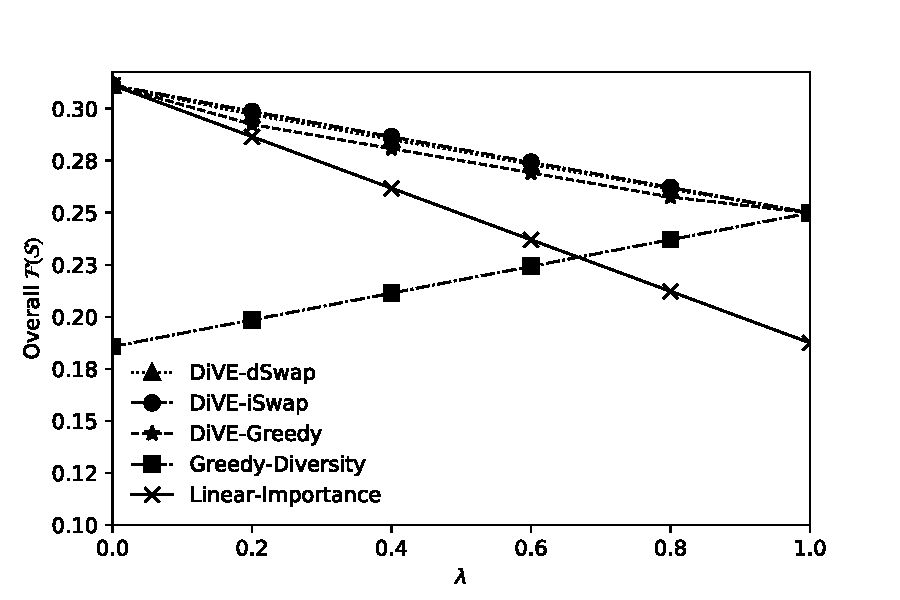
\includegraphics[width=2.6in]{figures/results/tradeoff_heart_2}
			\vspace{-15pt}
	\caption{Flights dataset}%, k = 5}
	\label{fig:impact_lambda_to_PI_sampling_greedy_pruning}
\end{figure}
}

\begin{figure}[t]
	\centering
	\subcaptionbox{Heart disease dataset}[.75\linewidth][c]{%
		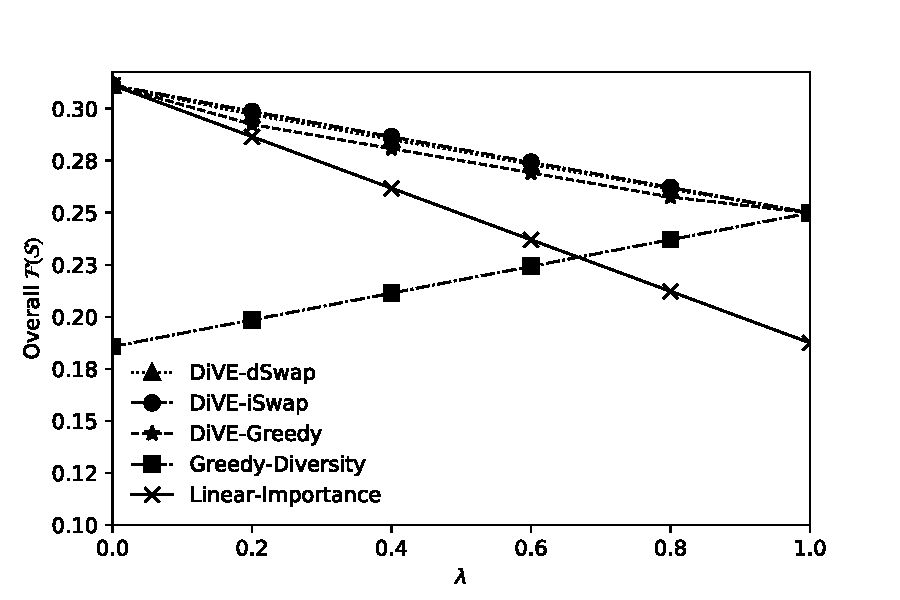
\includegraphics[width=.75\linewidth]{figures/results/tradeoff_heart_2}} \\
		\subcaptionbox{Flights dataset}[.75\linewidth][c]{%
		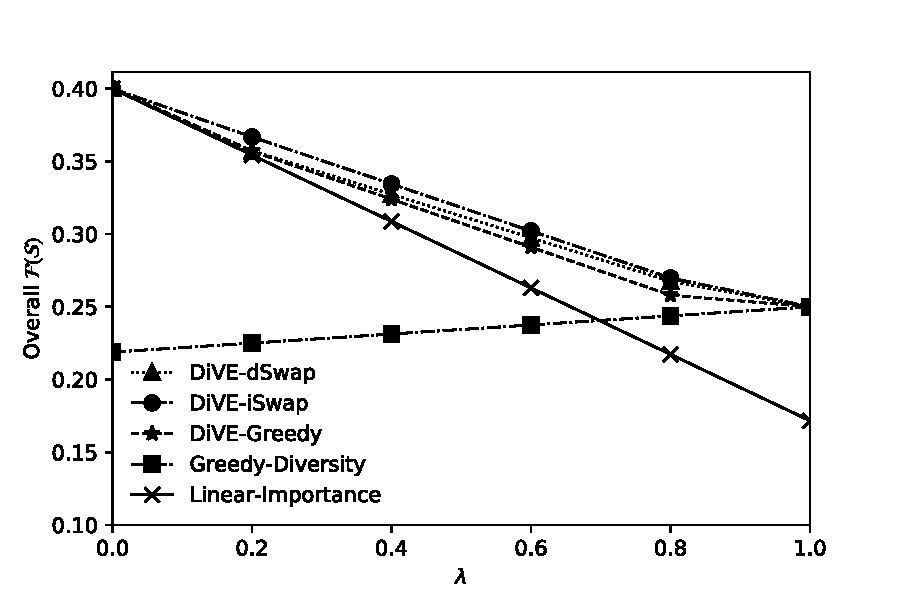
\includegraphics[width=.75\linewidth]{figures/results/tradeoff_flights}}
										\vspace{-10pt}				
	\caption{Impact of $\lambda$ on $F\left(S\right)$, k = 5}
	\label{fig:tradeoff_3_datasets}	
	\end{figure}



% The Impact of \lambda to the overall objective function value %


%\section{Experimental Evaluation}\label{sec:experimental_evaluation}

{\noindent{\bf The impact of $\lambda$ on $F$}:}
%The value of $\lambda$ balances the trade off between importance and diversity score. 
Figure \ref{fig:tradeoff_3_datasets} shows how the performance of each scheme in terms of $F\left(S\right)$ is effected as the value of  $\lambda$ varies from $0$ to $1$. Clearly, for the lower values of $\lambda$, the highest $F(S)$ is achieved by Linear-Importance. To the contrary, the Greedy-Diversity method achieves highest values of $F\left(S\right)$ as the $\lambda$ approaches $1$. 
Hence, there is a crossover between the two schemes. 
However, our proposed DiVE schemes have stable performance for all values of $\lambda$ and outperforms Linear-Importance and Greedy-Diversity. 


% The Impact of k to the overall objective function value %
\eat{
{\noindent{\bf The impact of k on $F$}:} 
Figure \ref{fig:objf_3_datasets} shows the $F\left(S\right)$ values for various schemes as the number of recommended views $k$ varies from $5$ to $35$. 
%
Overall the $F\left(S\right)$ value decreases with increasing value of $k$ for all the schemes. 
%
This is because both average importance score and diversity of a set $S$ decreases as new views are added to $S$. 
%
%The views added earlier to $S$ have higher importance score then the views added later. Similarly, the diversity function exhibits a diminishing marginal gain trend as the size of set $S$ increases. 
The important observation here is the fact that our {\em DiVE} schemes always have higher overall objective function values as compared to the two extreme baselines approaches for all values of $k$. 
%Among the {\em DiVE} schemes, DiVE-iSwap and DiVE-dSwap perform better than the Greedy versions. This is because, swap algorithm performs number of additional iterations to improve the value of the objective function.
\begin{figure}[t]
	\centering
	\subcaptionbox{Heart disease dataset}[.75\linewidth][c]{%
		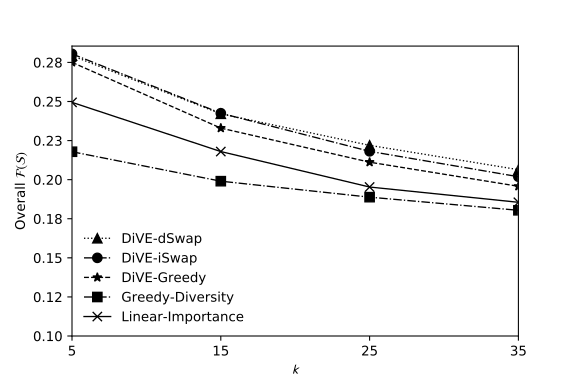
\includegraphics[width=.75\linewidth]{figures/results/objf_heart_2}} \\ 
	\subcaptionbox{Flights datasets}[.75\linewidth][c]{%
		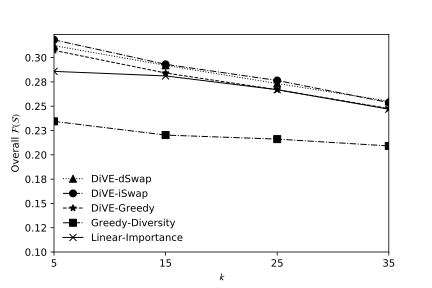
\includegraphics[width=.75\linewidth]{figures/results/objf_flights}}
								\vspace{-10pt}				
	\caption{Impact of k on $F\left(S\right)$, $\lambda = 0.5$}
	\label{fig:objf_3_datasets}
\end{figure}
}



%
%\begin{itemize}
%	\item Heart Disease Dataset \footnote{http://archive.ics.uci.edu/ml/datasets/heart+Disease}: This dataset is comprised of $9$ dimensional attributes and $5$ measure attributes. The number of possible views are $180$ with four aggregate functions.% and  has 14 attributes in total which are 9 attributes $ \mathbb{A} $ and 5 measure attributes $ \mathbb{M} $, $ \mathbb{A}  $= sex, cp, fbs, restecg, exang, slope, ca, thal, num; $ \mathbb{M} $ = age, trestbps, chol, thalach, oldpeak. This dataset has small number of rows (299 rows).
%	\item Airline (Flights) Dataset \footnote{http://stat-computing.org/dataexpo/2009/the-data.html}: This dataset is comprised of $7$ dimensional attributes and $4$ measure attributes. The number of possible views are $112$.%The detail as follows: $ \mathbb{A}  $= year, month, week, day, carrier, origin, destination; $ \mathbb{M}  $= arrivaldelay, departurdelay, weatherdelay, distance. This dataset has 855,632 number of rows. 
%\end{itemize}
%
%In particular, we evaluate the performance of following schemes:
%\begin{itemize}
%	\item Linear-Importance: Selects top-k views on the basis of only the importance score.
%	\item Greedy-Diversity: Selects top-k diverse views.
%	\item DiVE-Greedy: Selects top-k views on the basis of hybrid objective function using greedy algorithm.
%	\item DiVE-iSwap: Selects top-k views on the basis of hybrid objective function using swap algorithm initialized by Linear-importance method. 
%	\item DiVE-dSwap: Selects top-k views on the basis of hybrid objective function using swap algorithm initialized by Greedy-Diversity method.
%	\item Static-pruning: DiVE-Greedy and DiVE-dSwap methods using static pruning technique to reduce the number of view queries as presented in section \ref{dive-greedy-static}  and \ref{subsec:dive-dswap}
%	\item Adaptive-pruning: DiVE-Greedy and DiVE-dSwap methods using adaptive pruning method as discussed in section \ref{subsec:adaptive-pruning}.	
%\end{itemize}
%For each experiment a query workload of ten random queries is submitted to select ten different subsets of data $D_Q$. The performance measures are averaged over views recommended for each of those ten subsets. In particular, the performance of each scheme listed above is measured based on the following metrics:
%\begin{itemize}
%	\item {\bf  Interestingness of the views:} measured as the value of hybrid objective function 
%	$F\left(S\right)$ for selected set of views $S$, as defined in equation \ref{objectif_function}.
%	\item {\bf Total Cost:} measured as the sum of the cost to execute view queries and the cost to diversify the views that is : $C_T= C_Q + C_D$
%\end{itemize}


%\eat{
%	\textbf{\textit{Experimental Setup}}. This experiment running on Windows 10 64 bit, Intel Core i7-7700 CPU @ 3.60 GHz, RAM 16 GB. The experiment is developed using Python and run on Python version 3.6.3 with PostgreSQL as the database engine. Two real datasets are used, as follows: 
%}
%
%\eat{
%	\subsection{Effectiveness Evaluation}
%	%  Prolog of the quality of the results evaluation%
%	In order to test the performance of our proposed approach, we run experiments using two real datasets: flights dataset and heart disease dataset. For each dataset, we execute ten random queries. Afterwards, the average of all results is calculated as the final result. We examine the performance of our proposed schemes in term of the quality of the result (effectiveness) and the efficiency. All parameters used in this experiments are summarized in Table \ref{tab:tab-parameter} and the detail results of the experiments is elaborated next. 
%}